\documentclass[12pt,a4paper,oneside]{article}
\usepackage[utf8]{inputenc}
\usepackage{t1enc} % hyphenate accented chars
\usepackage[hungarian]{babel}
\usepackage{../fedlap}
\usepackage{fancyhdr} % elofej, elolab
\usepackage{graphicx}
\usepackage{datetime} % specify date format
\setcounter{secnumdepth}{3} % enable subsubsection

% hasonlitson a doc verziora
\addtolength{\voffset}{-1cm}

% cim
\csapat{nand}{39}
\konzulens{Bozóki Szilárd}
\datum{\todaynum}

% csapattagok
\taga{Berki Endre}{HQNHER}{berkiendre@gmail.com}
\tagb{Fodor Bertalan Ferenc}{H4T1UX}{foberci@gmail.com}
\tagc{Kádár András}{JFENWR}{arycika@gmail.com}
\tagd{Thaler Benedek}{EDDO10}{thalerbenedek@gmail.com}

\setlength{\headheight}{1.3em}
\setlength{\headsep}{2em}

% elofej, elolab
\fancyhf{}

\fancyhead[OL] { \tiny \leftmark{} }
\fancyhead[OR] { \tmpcsapat }

\fancyfoot[OR] { \thepage }
\fancyfoot[OL] { \tmpdatum }

\pagestyle{fancy}

% custom date format, according to customer request
% you have to use the \todaynum command instead of today,
% becouse babel overrides it, and I couldn't find a way to override
% it again. I was tempted to call this format \todaybozoki
\newcommand{\todaynum}{\the\year. \twodigit\month. \twodigit\day}


\begin{document}

\anyag{3. Analízis modell kidolgozása}
\fedlap

\addtocounter{section}{2}
\section{Analízis modell kidolgozása}

	\subsection{Objektum katalógus}
%GENERATOR:CLASS_RESPONSIBILITY
		\begin{description}
			\item[AbstractFrameItem] Alapértelmezett megvalósítása egy keretben lévő objektumnak.
			\item[Area] Területrészt leíró osztály. Összehasonlítható egy másik osztállyal, hogy fedik-e egymást.
			\item[DIRECTION] Irányokat jelöl a két dimenziós térben.
			\item[Door] Ajtó objektum, melyet ha megérint a Stickman úgy hogy az összes kulcs a birtokában van, az objektum a pálya teljesítettségét jelző eseményt bocsát ki.
			\item[Frame] A pálya által alkotott táblázat egy cellája, amely elemeket tartalmaz. Ez felelős az elemek (Stickman) mozgatásáért kereten belül és között egyaránt.
			\item[FrameItem] A keretben elhelyezkedő elemek által megvalósított iterfész, melyen keresztül a keret menedzselni tudja a benne lévő elemeket.
			\item[Game] A játékot reprezentáló objektum, amely kezeli az aktuális pályát.
			\item[Key] Kulcs elem, melyet megérintve a Stickman meg tud szerezni. Erről egy esemény küldésén keresztül értesíti a külvilágot.
			\item[Map] Számon tartja a pályán elhelyezett kulcsokat számát, valamint a már összegyűjtött kulcsok számát. Felelős a keretek mozgatásáért.
			\item[MapFactory] Felelős a pályák létrehozásáért, bennük a keretek és az elemek elhelyezéséért.
			\item[Platform] Olyan elem, mellyel nem tud a Stickman egy helyen tartózkodni, azaz korlátozza a Stickman mozgásterét.
			\item[PubSub] Üzenetközvetítő osztály, mely feliratkozásokat tart számon, és ha valakitől eseményt kap, arról értesíti az arra feliratkozottakat.
			\item[Stickman] A játékos által irányított figura, mely a pályán mozog.
			\item[Subscriber] Olyan interfész, melyen keresztül eseményeket lehet fogadni a PubSubtól.
			\item[Timer] Időzítésért felelős osztály, bizonyos időközönként kibocsát egy 'tick' eseményt az átadott PubSub objektumra.
		\end{description}
%GENERATOR:CLASS_RESPONSIBILITY	
	
	\subsection{Osztályok leírása}
	
%GENERATOR:CLASS_DESCRIPTIONS
		\subsubsection{AbstractFrameItem} Absztrakt osztály.
				 Alapértelmezett megvalósítása egy keretbe helyezett objektumnak.   Nyilvántartja a kereten belüli pozícióját, valamint hordoz  egy referenciát a tartalmazó keretre. 			\begin{description}


				\item[Ősosztályok] Object $\rightarrow{}$ AbstractFrameItem.
				\item[Interfészek] FrameItem.
				\item[Attribútumok]$\ $
					\begin{description}
						\item[\texttt{protected Area area}] A tartalmazó kereten belül elfoglalt pozíció 
						\item[\texttt{protected Frame frame}] A tartalmazó keret 
					\end{description}
				\item[Metódusok]$\ $
					\begin{description}
						\item[] (nincs)
					\end{description}
			\end{description}

		\subsubsection{Area}
				 Egy tetszőleges keret egy területét leíró osztály.  Ez az osztály elfedi, hogy egy keret valójában hány dimenziós,  valamint azt, hogy egy keret egy összefüggő ponthalmaza milyen   paraméterekkel írható le. 			\begin{description}


				\item[Ősosztályok] Object $\rightarrow{}$ Area.
				\item[Interfészek] (nincs)
				\item[Attribútumok]$\ $
					\begin{description}
						\item[\texttt{private int height}] A terület magassága 
						\item[\texttt{private int width}] A terület szélessége 
						\item[\texttt{private int x}] A terület bal felső sarkának x eltolása 
						\item[\texttt{private int y}] A terület bal felső sarkának y eltolása 
					\end{description}
				\item[Metódusok]$\ $
					\begin{description}
						\item[\texttt{public boolean hasCollision(Area area)}] \hfill \\ Ellenőrzi, hogy a kapott Area objektummal van-e közös pontja.  A metódus feltételezi, hogy a két terület azonos keretben található. 
					\end{description}
			\end{description}

		\subsubsection{DIRECTION}
				 Enumeráció. Elfedi, hogy a játéktér hány dimenziós.  A tartalmazott elemek leírják az összes lehetséges irányt,   melybe a játékos mozoghat, vagy keretet cserélhet.  			\begin{description}


				\item[Ősosztályok] Object $\rightarrow{}$ DIRECTION.
				\item[Interfészek] (nincs)
				\item[Attribútumok]$\ $
					\begin{description}
						\item[] (nincs)
					\end{description}
				\item[Metódusok]$\ $
					\begin{description}
						\item[] (nincs)
					\end{description}
			\end{description}

		\subsubsection{Door}
				 A pályák befejezésére szolgáló ajtót reprezentálja.  Ha a Stickman az összes kulcs birtokában megérinti,  a pálya teljesítésre kerül. 			\begin{description}


				\item[Ősosztályok] Object $\rightarrow{}$ AbstractFrameItem $\rightarrow{}$ Door.
				\item[Interfészek] (nincs)
				\item[Attribútumok]$\ $
					\begin{description}
						\item[] (nincs)
					\end{description}
				\item[Metódusok]$\ $
					\begin{description}
						\item[] (nincs)
					\end{description}
			\end{description}

		\subsubsection{Frame}
				 Egy pályán belüli keret, amelyben mozoghat a Stickman. Tartalmazza a pálya többi elemét (Door, Key, Platform). 			\begin{description}


				\item[Ősosztályok] Object $\rightarrow{}$ Frame.
				\item[Interfészek] (nincs)
				\item[Attribútumok]$\ $
					\begin{description}
						\item[] (nincs)
					\end{description}
				\item[Metódusok]$\ $
					\begin{description}
						\item[\texttt{public void addItem(FrameItem item)}] \hfill \\ Hozzáadja a megadott elemet a kerethez. 
						\item[\texttt{protected boolean checkCollision(Area area)}] \hfill \\ Ellenőrzi, hogy a megadott területen  található-e szilárd objektum. 
						\item[\texttt{protected boolean isTraversable(Frame frame)}] \hfill \\ Megállapítja, hogy a megadott kerettel  átjárható-e. 
						\item[\texttt{public void removeItem(FrameItem item)}] \hfill \\ Eltávolítja a megadott elemet a keretből 
						\item[\texttt{public boolean requestArea(FrameItem item, Area area)}] \hfill \\ A metódust hívó elem kérést intéz a kerethez,  hogy el szeretné foglalni a megadott területet.  A keret felelőssége a terület ellenőrzése, és szabad  terület esetén az elem pozíciójának frissítése. 
					\end{description}
			\end{description}

		\subsubsection{FrameItem} Interfész.
				 A Frame osztály ezen a felületen keresztül éri el a tartalmazott objektumokat.   Ezen interfacet valósítják meg a pályán lévő objektumok (Platform, Door, Key, Stickman) 			\begin{description}


				\item[Ősosztályok] Object $\rightarrow{}$ FrameItem.
				\item[Metódusok]$\ $
					\begin{description}
						\item[\texttt{public void collision(FrameItem colliding)}] \hfill \\ A tartalmazó keret jelezheti ezen a metóduson keresztül,  hogy egy másik elem, melyet paraméterül ad,  hozzáért (collision) ehez az elemhez. 
						\item[\texttt{public Area getArea()}] \hfill \\ Visszaadja az elem pozícióját a kereten belül. 
						\item[\texttt{public boolean isSolid()}] \hfill \\ Megadja, hogy az elem szilárd-e vagy sem.  Ez a kereten belüli mozgások esetén az  ütközések ellenőrzésekor használatos. 
						\item[\texttt{public void setArea(Area area)}] \hfill \\ Beállítja az elem pozícióját a kereten belül. 
						\item[\texttt{public void setFrame(Frame frame)}] \hfill \\ Beállítja az elemet tartalmazó keretet. 
					\end{description}
			\end{description}

		\subsubsection{Game}
				 A játékot szervező objektum. Felelős az új pályák betöltéséért és a teljesített pályák törléséért. 			\begin{description}


				\item[Ősosztályok] Object $\rightarrow{}$ Game.
				\item[Interfészek] (nincs)
				\item[Attribútumok]$\ $
					\begin{description}
						\item[\texttt{protected Map currentMap}] Az aktuális pálya 
					\end{description}
				\item[Metódusok]$\ $
					\begin{description}
						\item[\texttt{public void loadMap(int mapId)}] \hfill \\ Betölti a megadott pályát. 
					\end{description}
			\end{description}

		\subsubsection{Key}
				 A pályán található kulcsokat reprezentáló objektum. 			\begin{description}


				\item[Ősosztályok] Object $\rightarrow{}$ AbstractFrameItem $\rightarrow{}$ Key.
				\item[Interfészek] (nincs)
				\item[Attribútumok]$\ $
					\begin{description}
						\item[\texttt{private boolean collected}] Flag, ami jelzi, hogy megszerezték-e a kulcsot. 
					\end{description}
				\item[Metódusok]$\ $
					\begin{description}
						\item[\texttt{public boolean isCollected()}] \hfill \\ Megadja, hogy megszerezték-e a kulcsot. 
					\end{description}
			\end{description}

		\subsubsection{Map}
				 A pályákat reprezentálja. Tartalmazza a kereteket és azok elhelyezkedését,  kontrolállja az átrendezésüket. 			\begin{description}


				\item[Ősosztályok] Object $\rightarrow{}$ Map.
				\item[Interfészek] (nincs)
				\item[Attribútumok]$\ $
					\begin{description}
						\item[] (nincs)
					\end{description}
				\item[Metódusok]$\ $
					\begin{description}
						\item[\texttt{public void addItem(FrameItem item)}] \hfill \\ Hozzáadja a megadott elemet az elem által specifikált pozícióhoz.  Amennyiben a pálya inicializálása során az adott helyen még nincs keret,  létrehoz egyet.   A hozzáadott elem pozícióját megváltoztatja úgy, hogy az relatív  legyen a tartalmazó kerethez. 
						\item[\texttt{public Frame getNeighbour(Frame caller, DIRECTION direction)}] \hfill \\ Visszaadja a megadott keret direction irányba található  szomszédját. null-t ad vissza, ha a megadott irányban  nincs szomszéd. 
					\end{description}
			\end{description}

		\subsubsection{MapFactory}
				 Azonosító alapján Pályákat szolgáltat.  Létrehozza a pályát, majd az azonosító alapján feltölti  a megfelelő objektumokkal. 			\begin{description}


				\item[Ősosztályok] Object $\rightarrow{}$ MapFactory.
				\item[Interfészek] (nincs)
				\item[Attribútumok]$\ $
					\begin{description}
						\item[] (nincs)
					\end{description}
				\item[Metódusok]$\ $
					\begin{description}
						\item[\texttt{public Map getMap(int mapId, PubSub ps)}] \hfill \\ Létrehozza a megadott azonosítójú pályát  és feltölti elemekkel. 
					\end{description}
			\end{description}

		\subsubsection{Platform}
				 A Stickman és ezzel a játék mozgásterét korlátozó elem. A framen belül bejárható rész keretezésére szolgál. 			\begin{description}


				\item[Ősosztályok] Object $\rightarrow{}$ AbstractFrameItem $\rightarrow{}$ Platform.
				\item[Interfészek] (nincs)
				\item[Attribútumok]$\ $
					\begin{description}
						\item[] (nincs)
					\end{description}
				\item[Metódusok]$\ $
					\begin{description}
						\item[] (nincs)
					\end{description}
			\end{description}

		\subsubsection{PubSub}
				 Üzenetközvetítő csatorna, mely a Publish/Subscribe mintát valósítja meg. 			\begin{description}


				\item[Ősosztályok] Object $\rightarrow{}$ PubSub.
				\item[Interfészek] (nincs)
				\item[Attribútumok]$\ $
					\begin{description}
						\item[] (nincs)
					\end{description}
				\item[Metódusok]$\ $
					\begin{description}
						\item[\texttt{public void emit(String eventName, Object data)}] \hfill \\ Esemény publikálása 
						\item[\texttt{public void on(String eventName, Subscriber callback)}] \hfill \\ Feliratkozás eseményre 
					\end{description}
			\end{description}

		\subsubsection{Stickman}
				 A játékos által irányított figurát reprezentáló elem. 			\begin{description}


				\item[Ősosztályok] Object $\rightarrow{}$ AbstractFrameItem $\rightarrow{}$ Stickman.
				\item[Interfészek] (nincs)
				\item[Attribútumok]$\ $
					\begin{description}
						\item[] (nincs)
					\end{description}
				\item[Metódusok]$\ $
					\begin{description}
						\item[\texttt{private Area getNewAreaByDirection(DIRECTION direction)}] \hfill \\ A figura igényelt elmozdulása után elfoglalandó  terület kiszámítása. 
						\item[\texttt{public void move(DIRECTION direction)}] \hfill \\ A figura mozgatása a megadott irányba. 
						\item[\texttt{public void resetToCheckpoint()}] \hfill \\ A figura pozíciójának visszaállítása az  utolsó ellenőrzőpontra. 
					\end{description}
			\end{description}

		\subsubsection{Subscriber} Interfész.
				 A PubSub objektumnak átadható eseménykezelő felülete. 			\begin{description}


				\item[Ősosztályok] Object $\rightarrow{}$ Subscriber.
				\item[Metódusok]$\ $
					\begin{description}
						\item[\texttt{public void eventEmitted(String eventName, Object eventParameter)}] \hfill \\ A PubSub objektum által meghívott metódus,  a feliratkozott esemény bekövetkeztekor. 
					\end{description}
			\end{description}

		\subsubsection{Timer}
				 Az idő múlását nyilvántartó objektum.   Elsősorban Stickman esését szabályozhatjuk vele, de a  periodikus időközönként kiadott 'tick' események  a stickmentől vagy bármely más objektumtól függetlenek.  			\begin{description}


				\item[Ősosztályok] Object $\rightarrow{}$ Timer.
				\item[Interfészek] (nincs)
				\item[Attribútumok]$\ $
					\begin{description}
						\item[\texttt{ PubSub pubsub}] Az eseménykezelő csatorna,  melyen jelzi az idő múlását. 
					\end{description}
				\item[Metódusok]$\ $
					\begin{description}
						\item[] (nincs)
					\end{description}
			\end{description}

%GENERATOR:CLASS_DESCRIPTIONS

	\subsection{Statikus struktúra diagramok}

		\begin{center}
			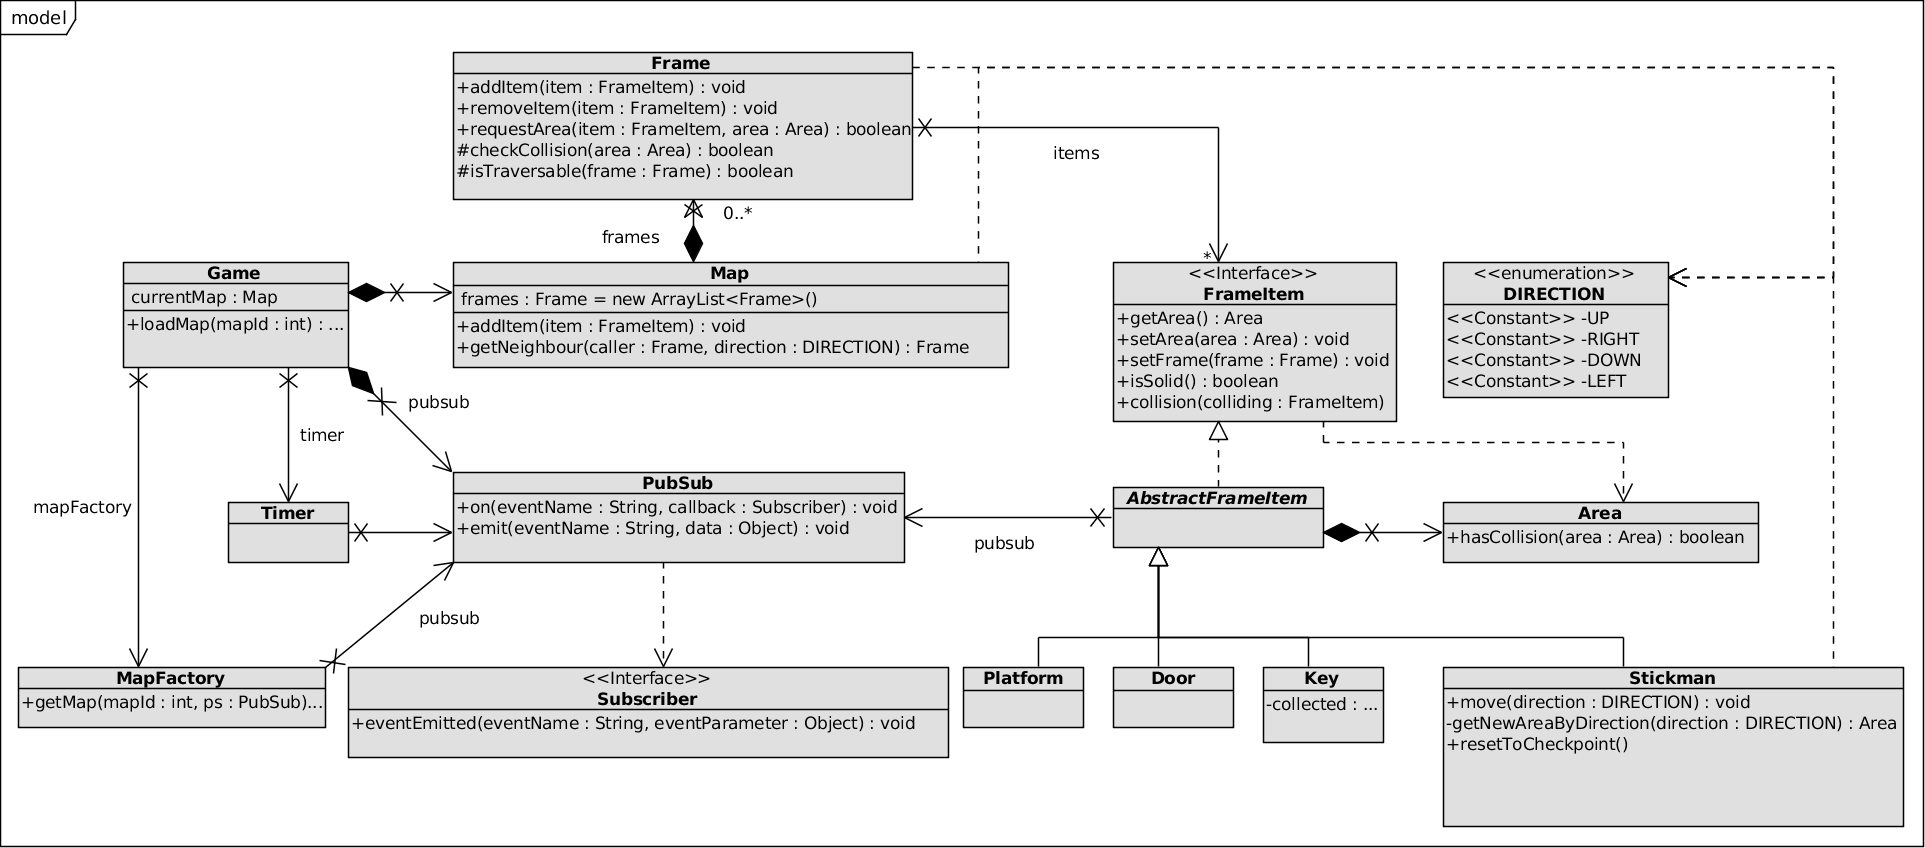
\includegraphics[scale=0.7, angle=-90]{resources/model.png}
		\end{center}
			
	\subsection{Szekvencia diagramok}
	
\begin{center}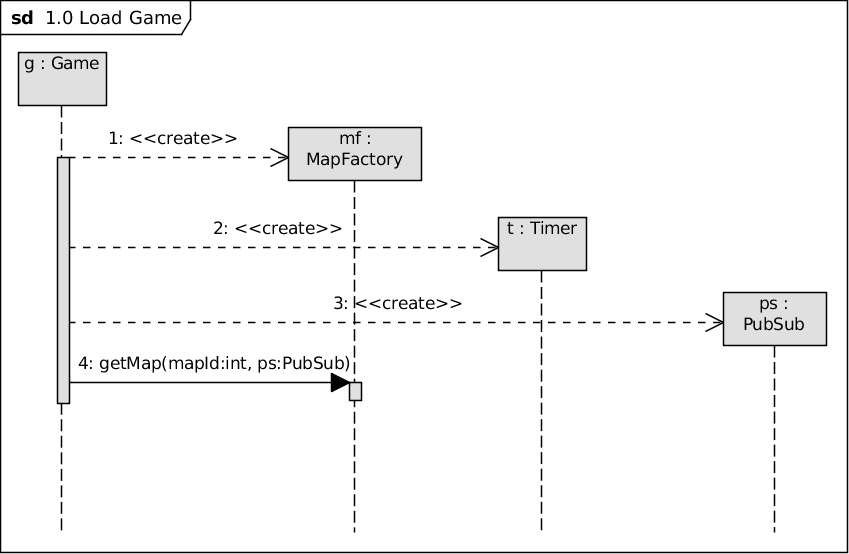
\includegraphics[scale=1]{resources/10LoadGame.png}\end{center}
\begin{center}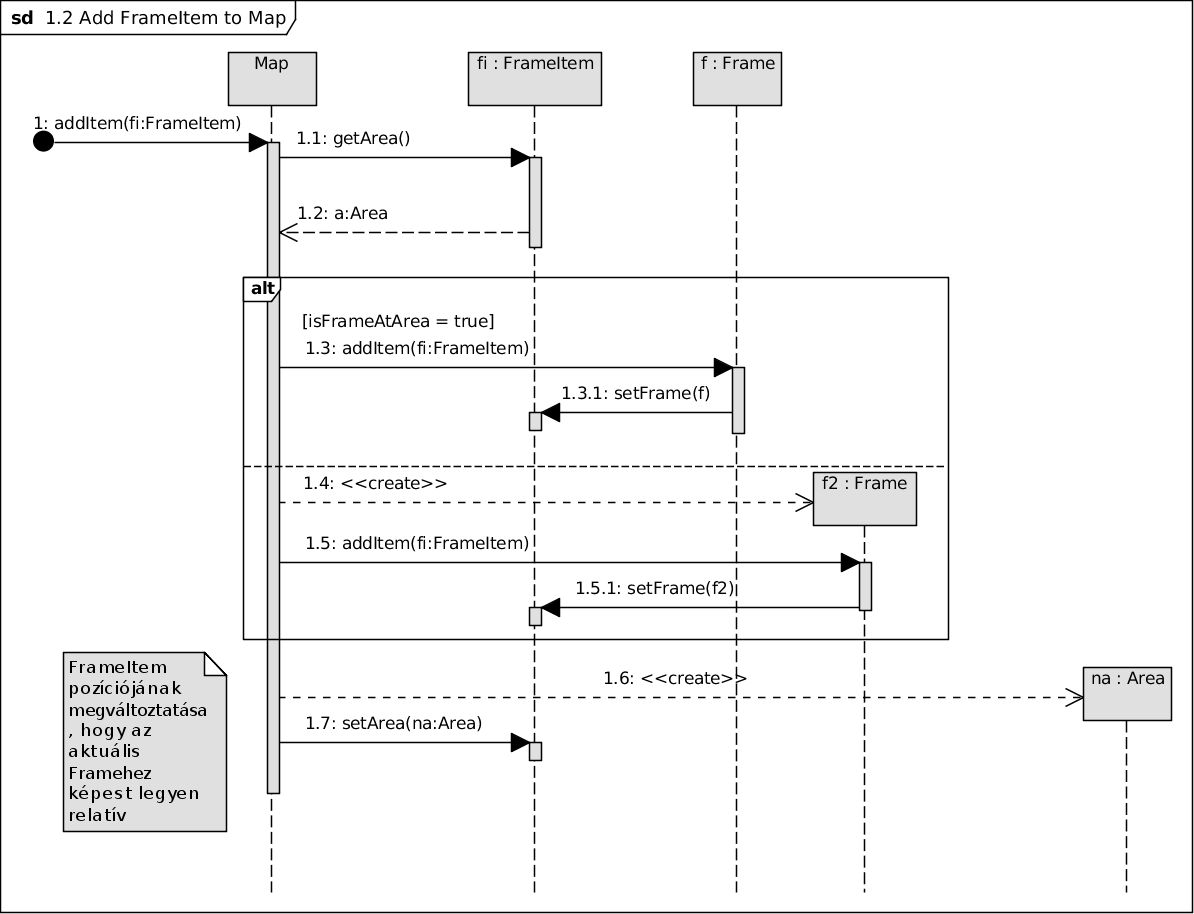
\includegraphics[scale=0.8]{resources/12AddFrameItemtoMap.png}\end{center}
\begin{center}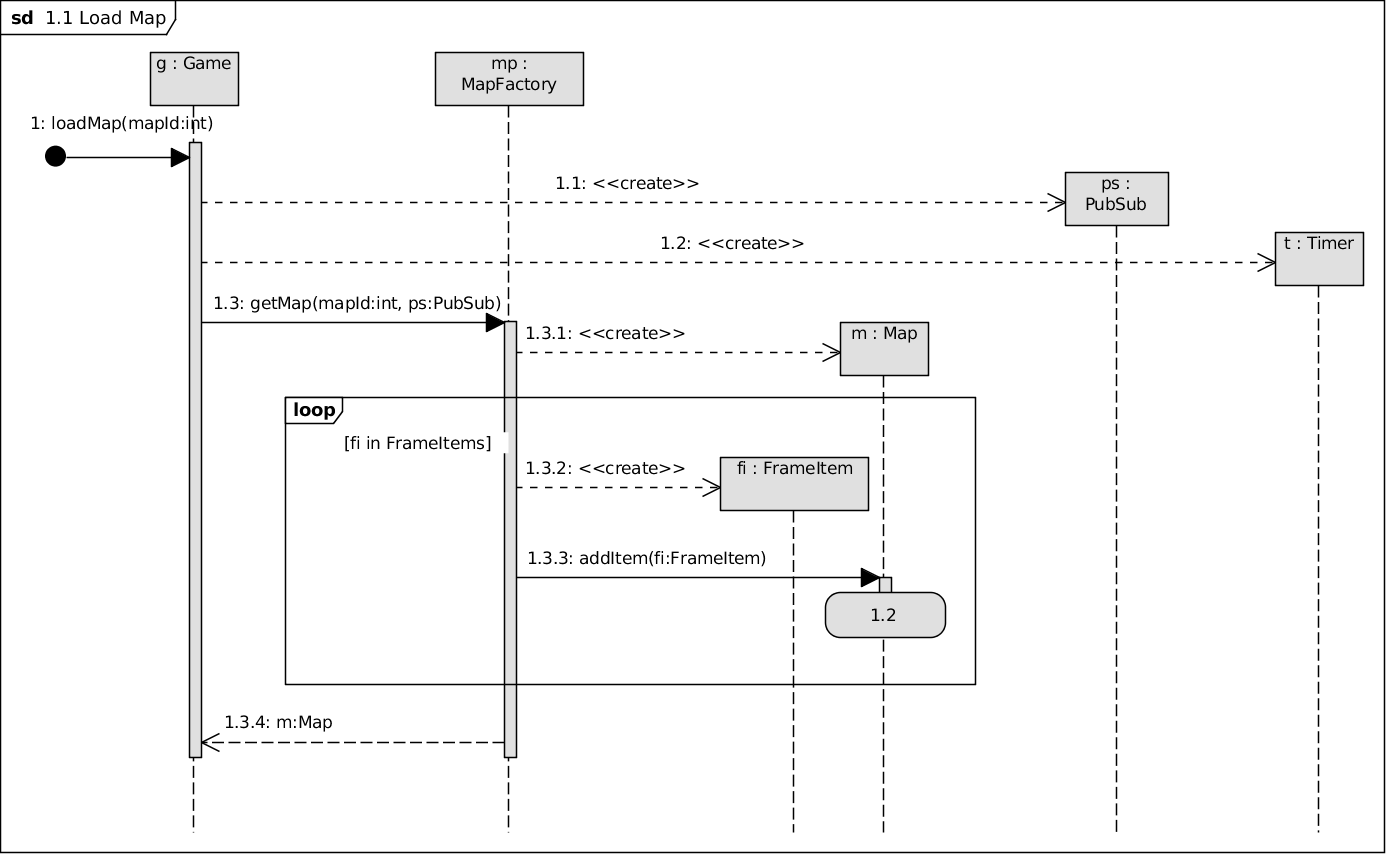
\includegraphics[scale=1, angle=-90]{resources/11LoadMap.png}\end{center}
\begin{center}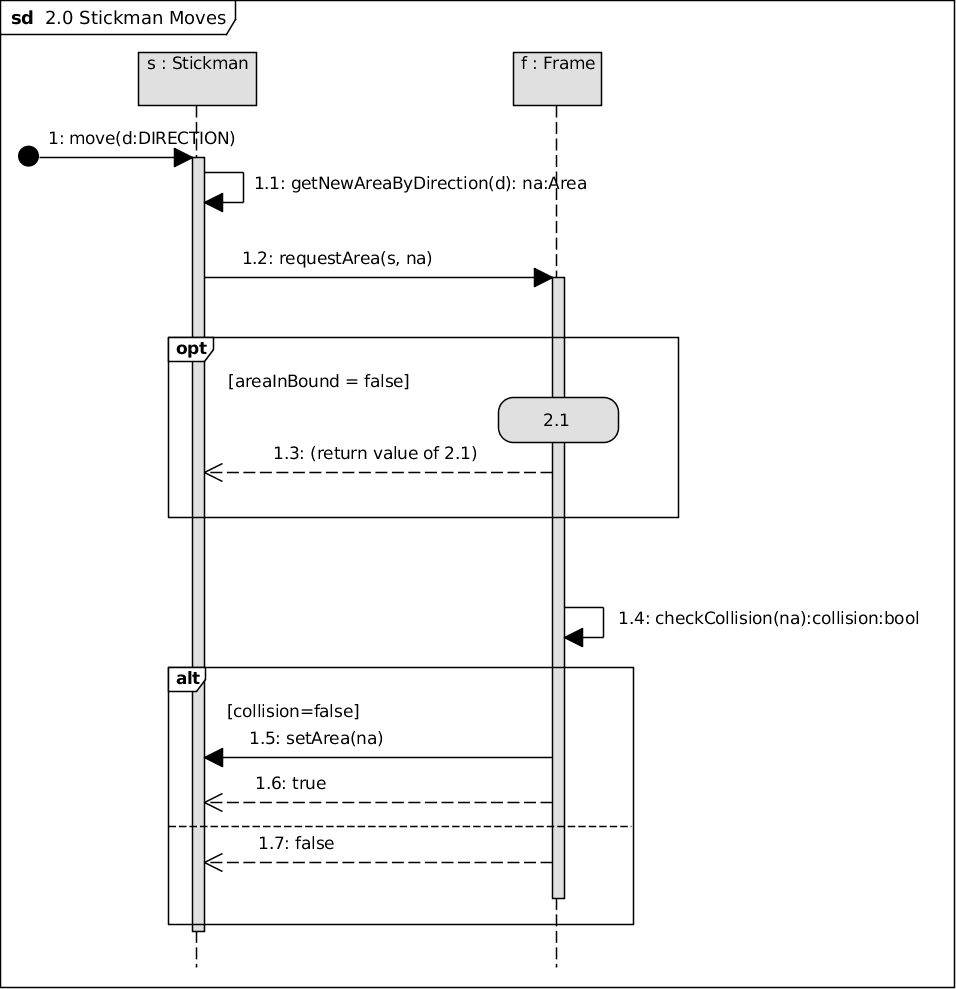
\includegraphics[scale=1]{resources/20StickmanMoves.png}\end{center}
\begin{center}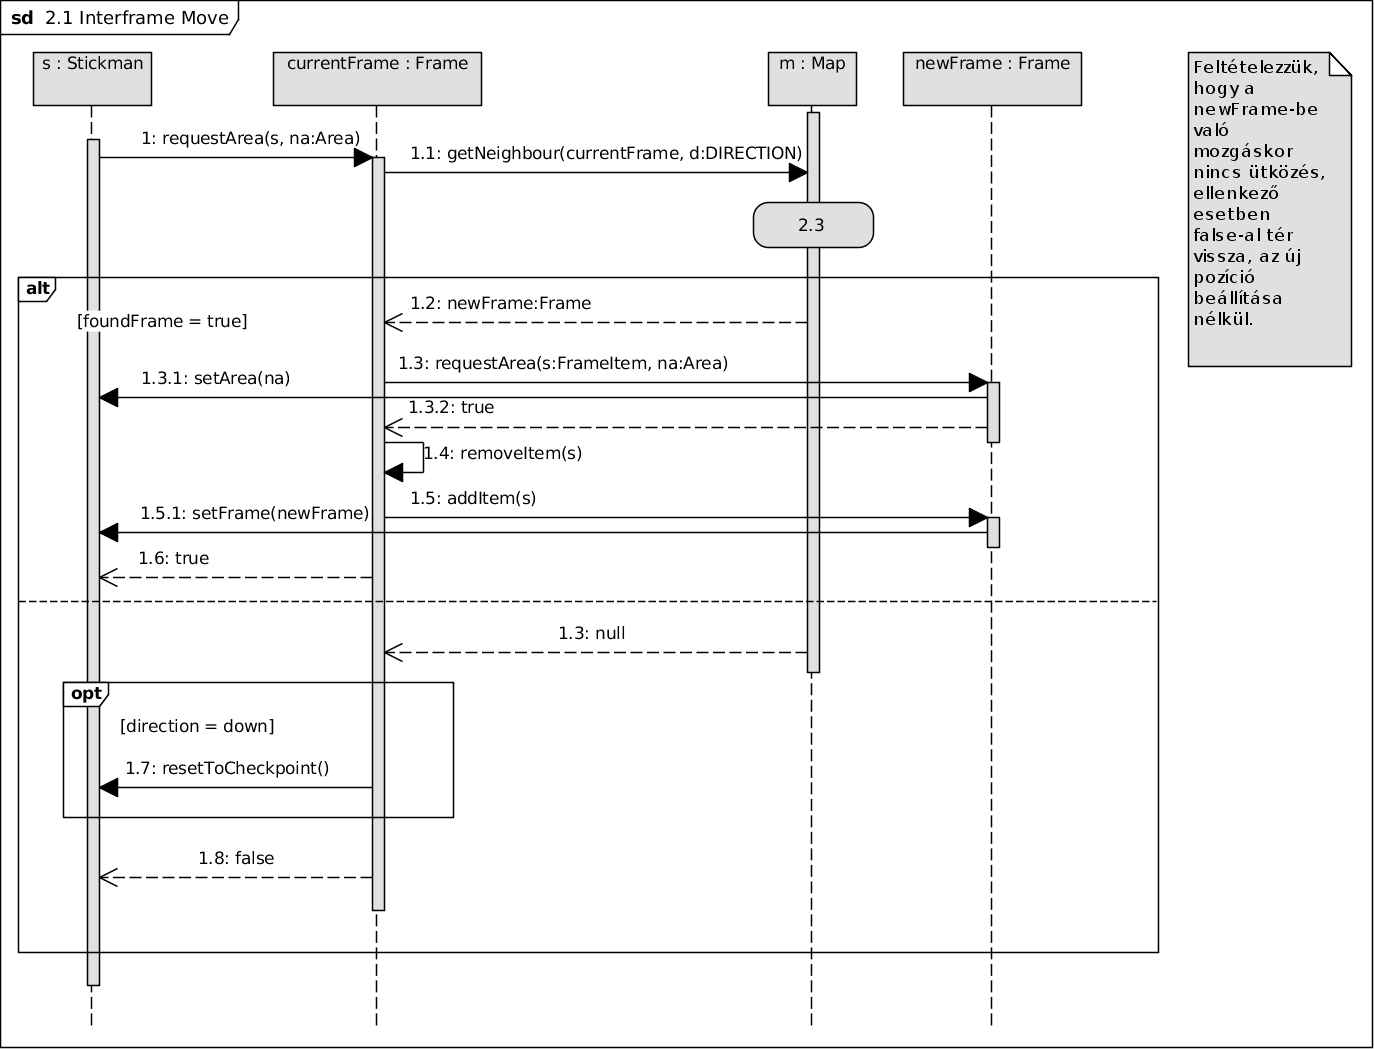
\includegraphics[scale=0.8, angle=-90]{resources/21InterframeMove.png}\end{center}
\begin{center}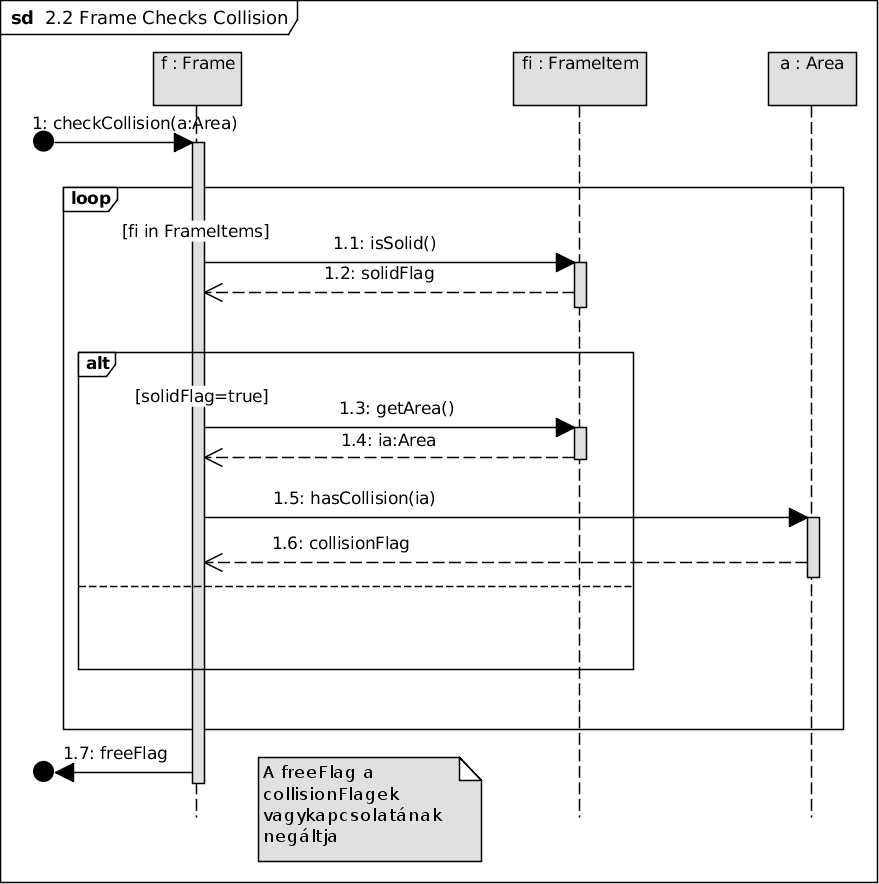
\includegraphics[scale=1]{resources/22FrameChecksCollision.png}\end{center}
\begin{center}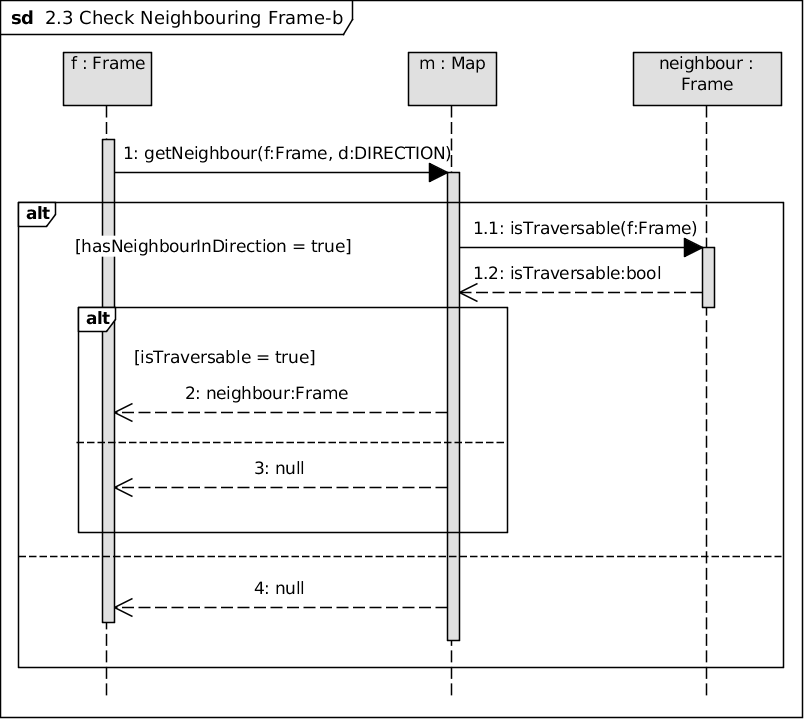
\includegraphics[scale=1]{resources/23CheckNeighbouringFrame.png}\end{center}
\begin{center}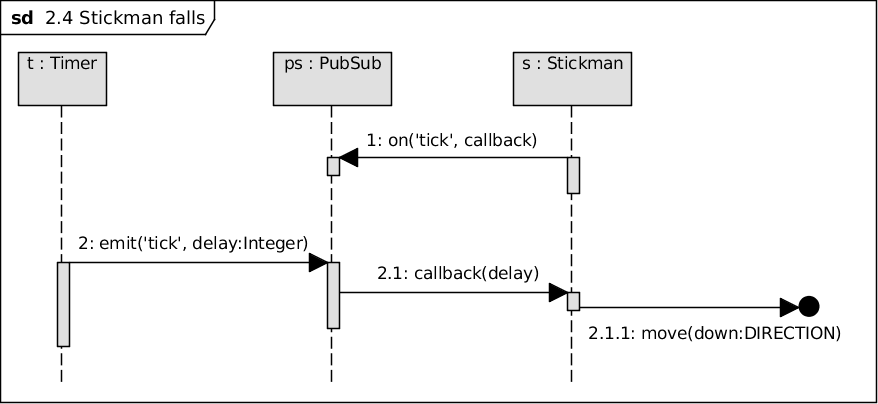
\includegraphics[scale=1]{resources/24Stickmanfalls.png}\end{center}
\begin{center}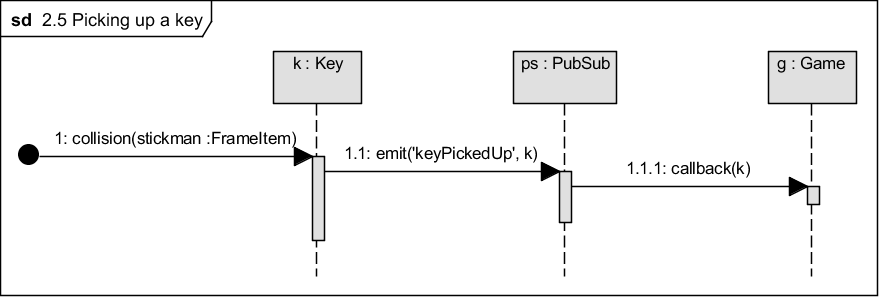
\includegraphics[scale=1]{resources/25PickingUpKey.png}\end{center}
\begin{center}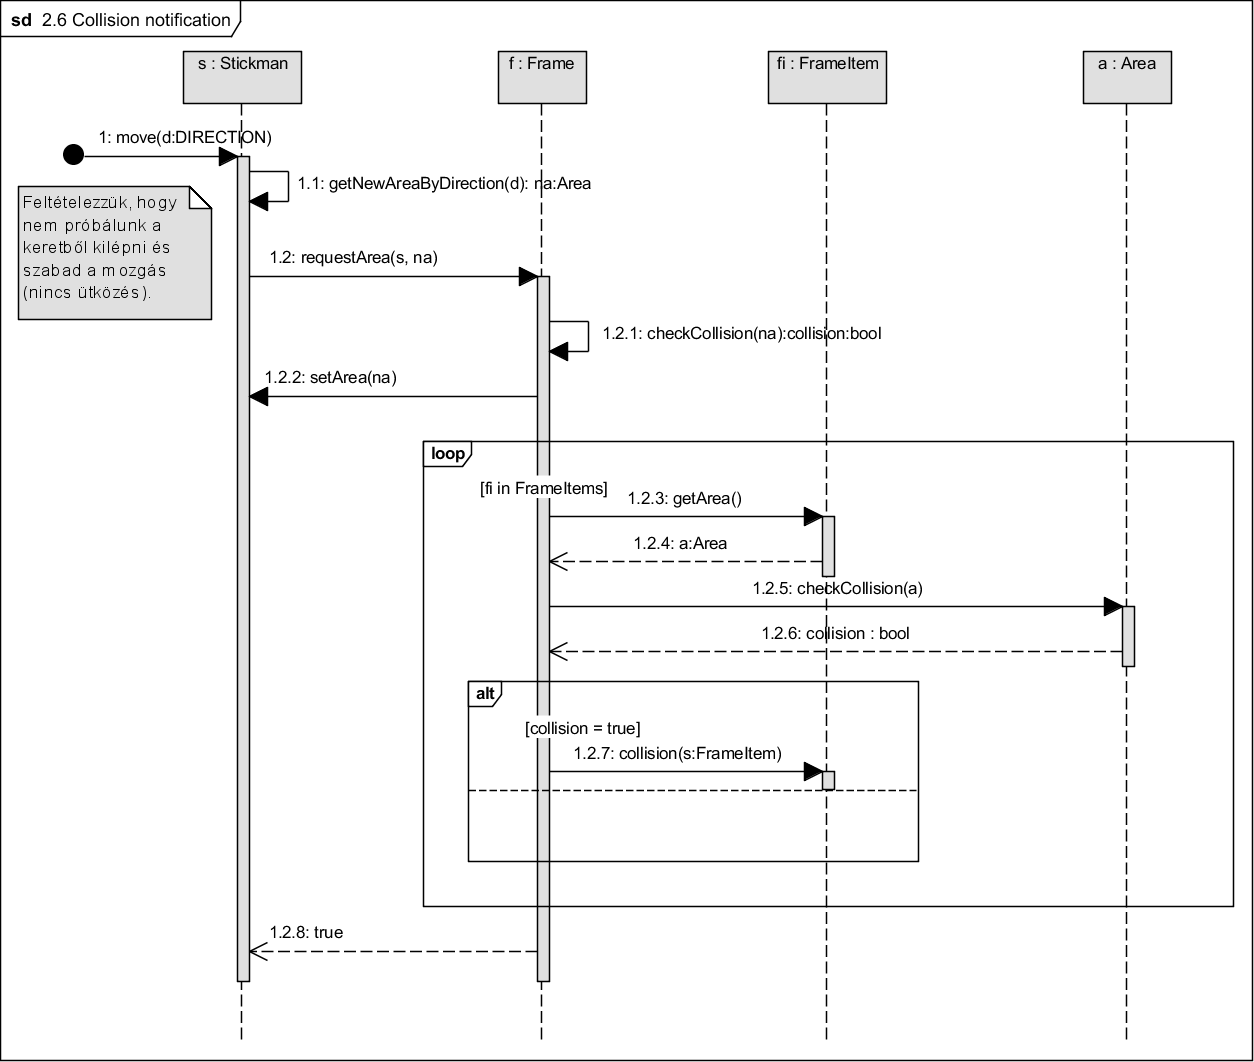
\includegraphics[scale=0.8, angle=-90]{resources/26CollisionNotification.png}\end{center}

	\subsection{State-chartok}
\begin{center}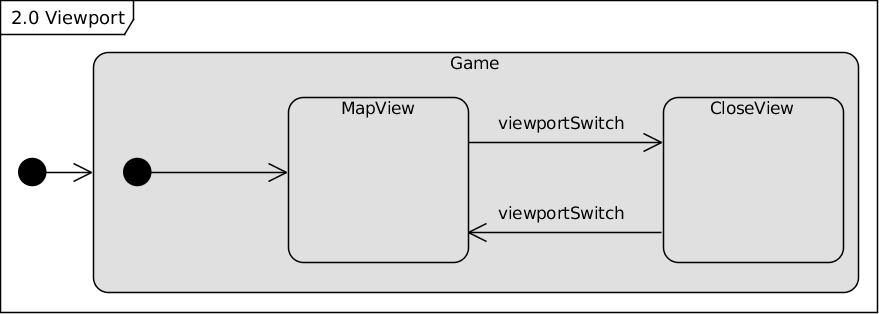
\includegraphics[scale=1]{resources/20Viewport.png}\end{center}
\begin{center}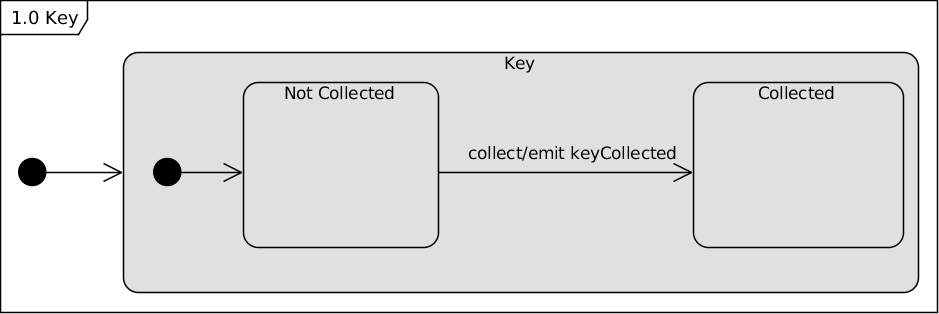
\includegraphics[scale=1]{resources/10Key.png}\end{center}	

	
	\subsection{Napló}
	% The diary generator uses the following comments to identify the beginning and the ending of the generated diary
	% The following content is auto generated, please do NOT modify, edit the related shared document instead.
	%GENERATOR:DIARY
    \begin{center} 
        \begin{tabular}{| l | p{1.9cm} | p{2.6cm} | p{6.1cm} |}
            \hline
                Kezdet & Időtartam & Résztvevők & Leírás \\
            \hline \hline 
2012. 02. 21. 20:00 & 1 óra & Fodor & Visual Paradigm modellező eszköz lehetőségeinek felmérése\\ \hline
2012. 02. 22. 12:00 & 0.5 óra & Értekezlet & Második fázis feladatainak megbeszélése. Döntés: Thaler közzéteszi a munkák alapját adó UML diagramot\\ \hline
2012. 02. 22. 18:30 & 1.5 óra & Thaler & 03. latex gerinc, korábbi hibák javítása\\ \hline
2012. 02. 22. 20:00 & 0.5 óra & Thaler & *.vpp fájlok verziókezelési lehetőségeinek vizsgálata\\ \hline
2012. 02. 22. 20:00 & 1.5 óra & Fodor & Eclipse - VP integráció vizsgálata\\ \hline
2012. 02. 22. 20:30 & 2 óra & Thaler & Class és Szekv. diagramok készítése\\ \hline
2012. 02. 22. 8:00 & 1.5 óra & Fodor, Kádár, Thaler & Konzultáció\\ \hline
2012. 02. 23. 15:30 & 3 óra & Kádár & Java kód generálás, dokumentálás\\ \hline
2012. 02. 23. 19:00 & 1.5 óra & Thaler & Sequence diagramok készítése\\ \hline
2012. 02. 23. 20:00 & 2 óra & Fodor & Modellezés\\ \hline
2012. 02. 25. 15:00 & 3 óra & Thaler & Sequence diagramok készítése\\ \hline
2012. 02. 26. 08:00 & 1.5 óra & Kádár & Beadandó dokumentum átnézése, nyomtatása\\ \hline
2012. 02. 26. 11:00 & 1 óra & Thaler & Sequence diagramok készítése\\ \hline
2012. 02. 26. 13:30 & 1.5 óra & Thaler & Class diagram készítése\\ \hline
2012. 02. 26. 15:00 & 2.5 óra & Thaler & JavaToLatex tool szerkesztése\\ \hline
2012. 02. 26. 17:30 & 1.5 óra & Thaler & Osztályok dokumentálása\\ \hline
2012. 02. 26. 18:00 & 7 óra & Fodor & Modellezés, Diagramok átnézése/kiegészítése, felelősségek dokumentálása\\ \hline
2012. 02. 26. 19:30 & 2 óra & Thaler & Modellezés\\ \hline
2012. 02. 26. 20:00 & 1 óra & Berki & UML -> PNG transzformáció és latex beillesztés\\ \hline
2012. 02. 26. 21:30 & 1 óra & Thaler & javaToLatex tool autoinsert\\ \hline
2012. 02. 26. 22:20 & 3 óra & Kádár & UML to vektorformátum\\ \hline
2012. 02. 26. 22:30 & 2.5 óra & Thaler & Generált tartalmak beillesztése, tisztítás, napló\\ \hline

            \hline
        \end{tabular}
    \end{center}
%GENERATOR:DIARY
\end{document}
